%! Author = Filippo Vissani
%! Date = 08/02/24
% !TeX root = ../thesis-main.tex

%----------------------------------------------------------------------------------------
\chapter{Analysis}
\label{chap:analysis}
%----------------------------------------------------------------------------------------
\section{State of the Art}

\subsection{Protelis}

Protelis~\cite{Pianini2015} is based on field calculus and is closely related to Proto~\cite{Beal2006}. It inherits spatial computing features from the field calculus, which provides universality, consistency, and self-stabilization properties. However, Protelis improves over Proto by offering a richer API through Java integration, support for code mobility through first-order functions, and a syntax inspired by C-family languages.

The syntax of Protelis (\Cref{fig:protelis-syntax}) is presented in abstract form. It uses meta-variables to represent names of user-defined functions (\texttt{f}), variables and function arguments (\texttt{x}), literal values (l), built-in functions and operators (b), Java method names (\texttt{m}), and aliases of static Java methods (\texttt{\#a}). The syntax employs conventions like comma-separated lists and semi-colon separators for sequences of elements.

Protelis adopts a familiar C- or Java-like syntax, making it more accessible and reducing barriers to adoption. Despite its syntactic similarity to imperative languages, Protelis is purely functional. Programs consist of a sequence of function definitions, followed by a main block of statements. Functions are defined with curly brackets and can contain sequences of statements or expressions. Each statement is an expression to be evaluated (\texttt{e}), possibly in the context of the creation of a new variable (\texttt{let x = e}) or a re-assignment (\texttt{x = e}).

\begin{figure}
    \centering
    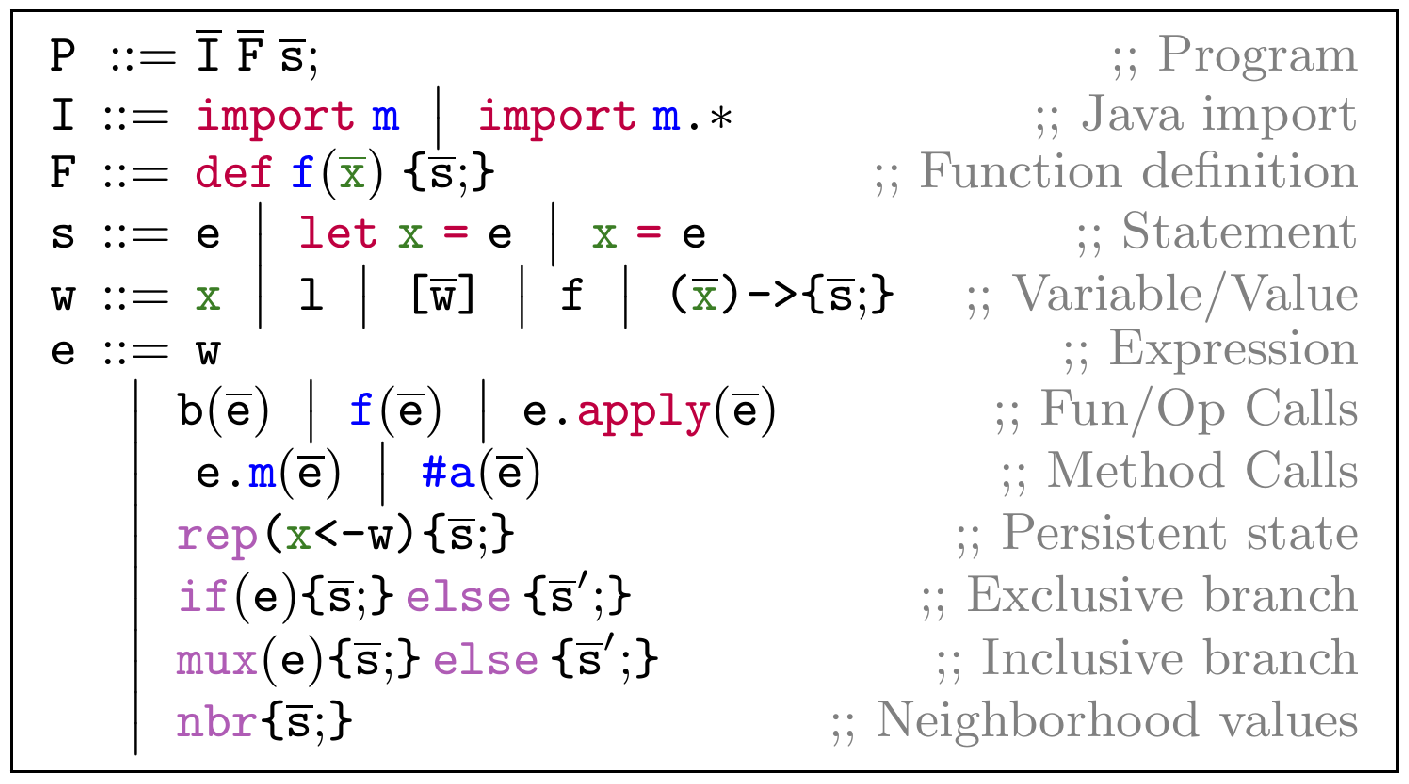
\includegraphics[width=.8\linewidth]{figures/protelis-syntax.png}
    \caption{Protelis abstract syntax}
    \label{fig:protelis-syntax}
\end{figure}

\subsubsection{Example: Rendezvous at a Mass Event}

In large public events, it can be challenging to meet with companions due to crowded areas, inaccessible rendezvous points, or difficulty in accessing cloud-based services.

Utilizing peer-to-peer geometric calculations across a network of devices to compute a \textit{rendezvous}\footnote{A meeting at an agreed time and place.} route is the proposed solution to the problem. The solution is demonstrated in a simulated city center environment (\Cref{fig:protelis-example-map}), using London as an example, with devices distributed randomly across the city streets. Each device has a communication range, and the goal is for two individuals (represented by their devices) to meet at a specific location.

The implementation (\Cref{lst:protelis-example}) involves injecting the environment of the devices with properties representing their owners (e.g., "Alice" and "Bob"). The algorithm measures the distance to one of the participants, creates a potential field, and builds an optimal path from the other participant, descending the distance potential field to reach the first participant at zero distance. The algorithm utilizes two main functions: \texttt{distanceTo} and \texttt{descend}. \texttt{distanceTo} measures the distance to one of the participants. Given a device and a potential field, \texttt{descend} builds a path of devices connecting the device with the source of the potential field. The algorithm elegantly compresses the entire process into a few lines of code, utilizing the \texttt{nbr} operator to exchange required information without explicitly declaring any communication protocol.

As \Cref{fig:protelis-example-map} shows, the simulation rapidly identifies a chain of devices (represented by red dots) that marks a sequence of waypoints for both device owners to walk and meet in the middle. The algorithm dynamically adjusts the path if one of the device owners moves in a different direction, ensuring it continues to recommend the best path for rendezvous.

\lstinputlisting[float,label={lst:protelis-example},caption=Rendezvous implementation in Protelis]{listings/protelis-example.txt}

\begin{figure}
    \centering
    \begin{subfigure}[b]{.49\textwidth}
        \centering
        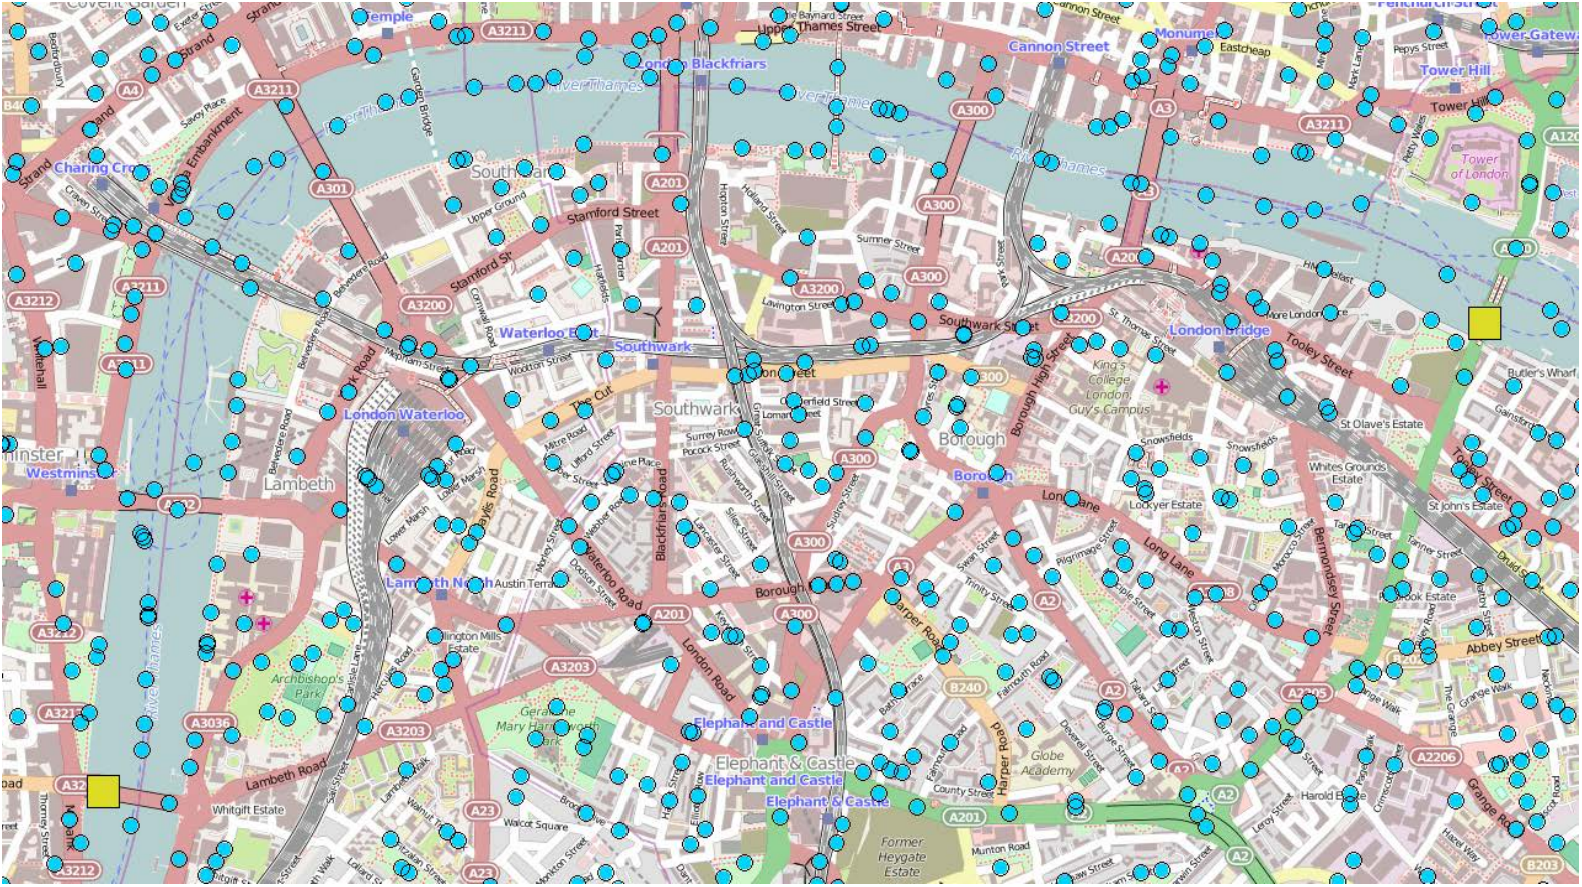
\includegraphics[width=\textwidth]{figures/protelis-example-a.png}
        \caption{Initial configuration.}
        \label{fig:protelis-example-a}
    \end{subfigure}
    \hfill
    \begin{subfigure}[b]{.49\textwidth}
        \centering
        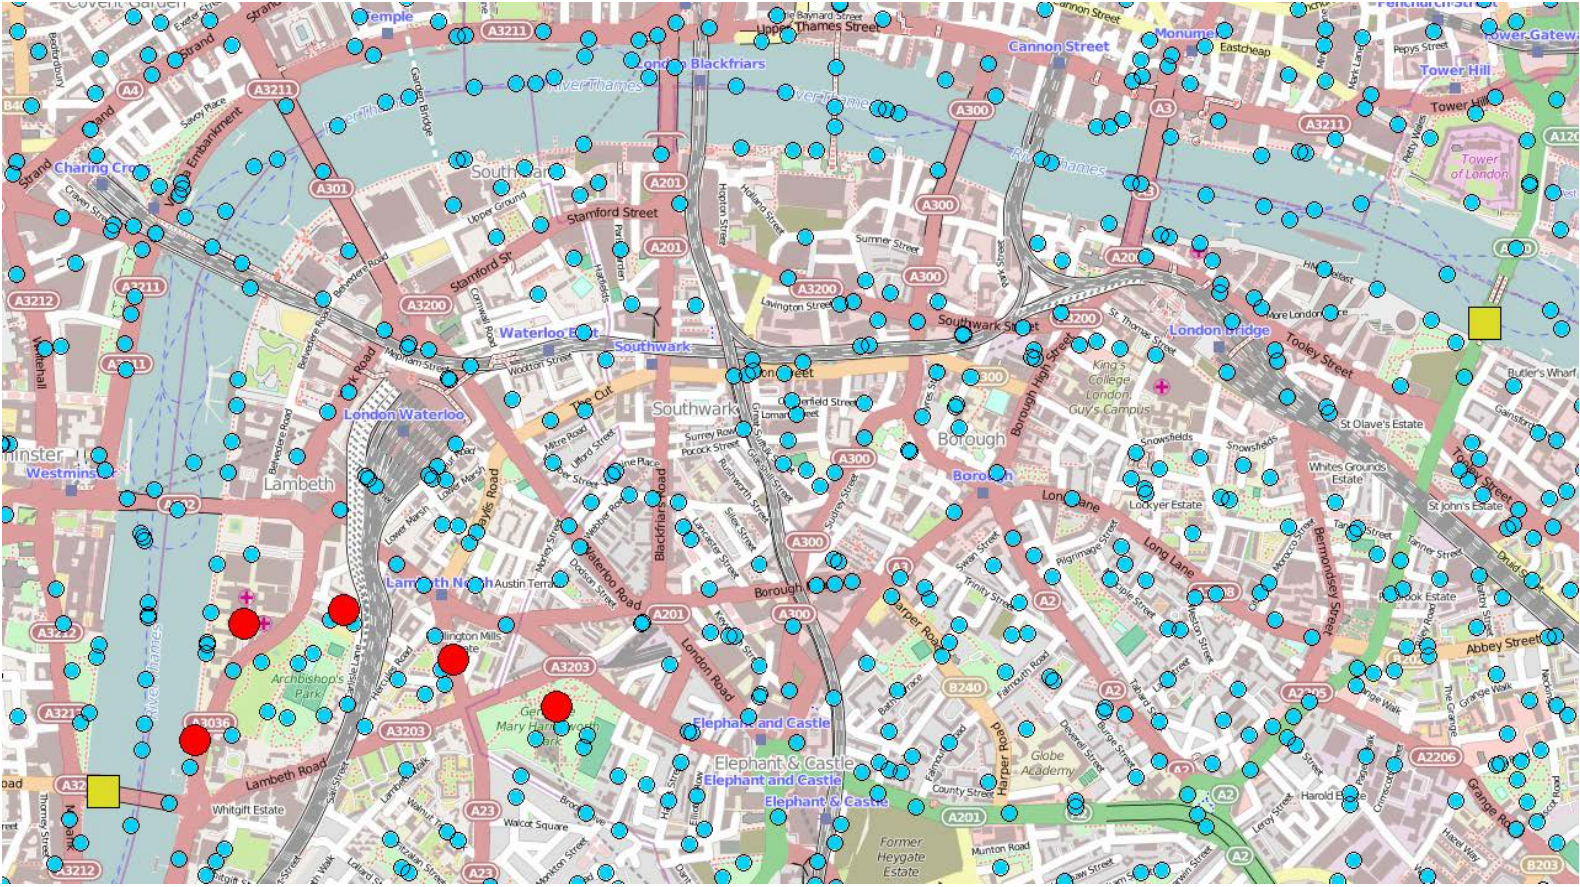
\includegraphics[width=\textwidth]{figures/protelis-example-b.png}
        \caption{Path begins to form.}
        \label{fig:protelis-example-b}
    \end{subfigure}
    \hfill
    \begin{subfigure}[b]{.49\textwidth}
        \centering
        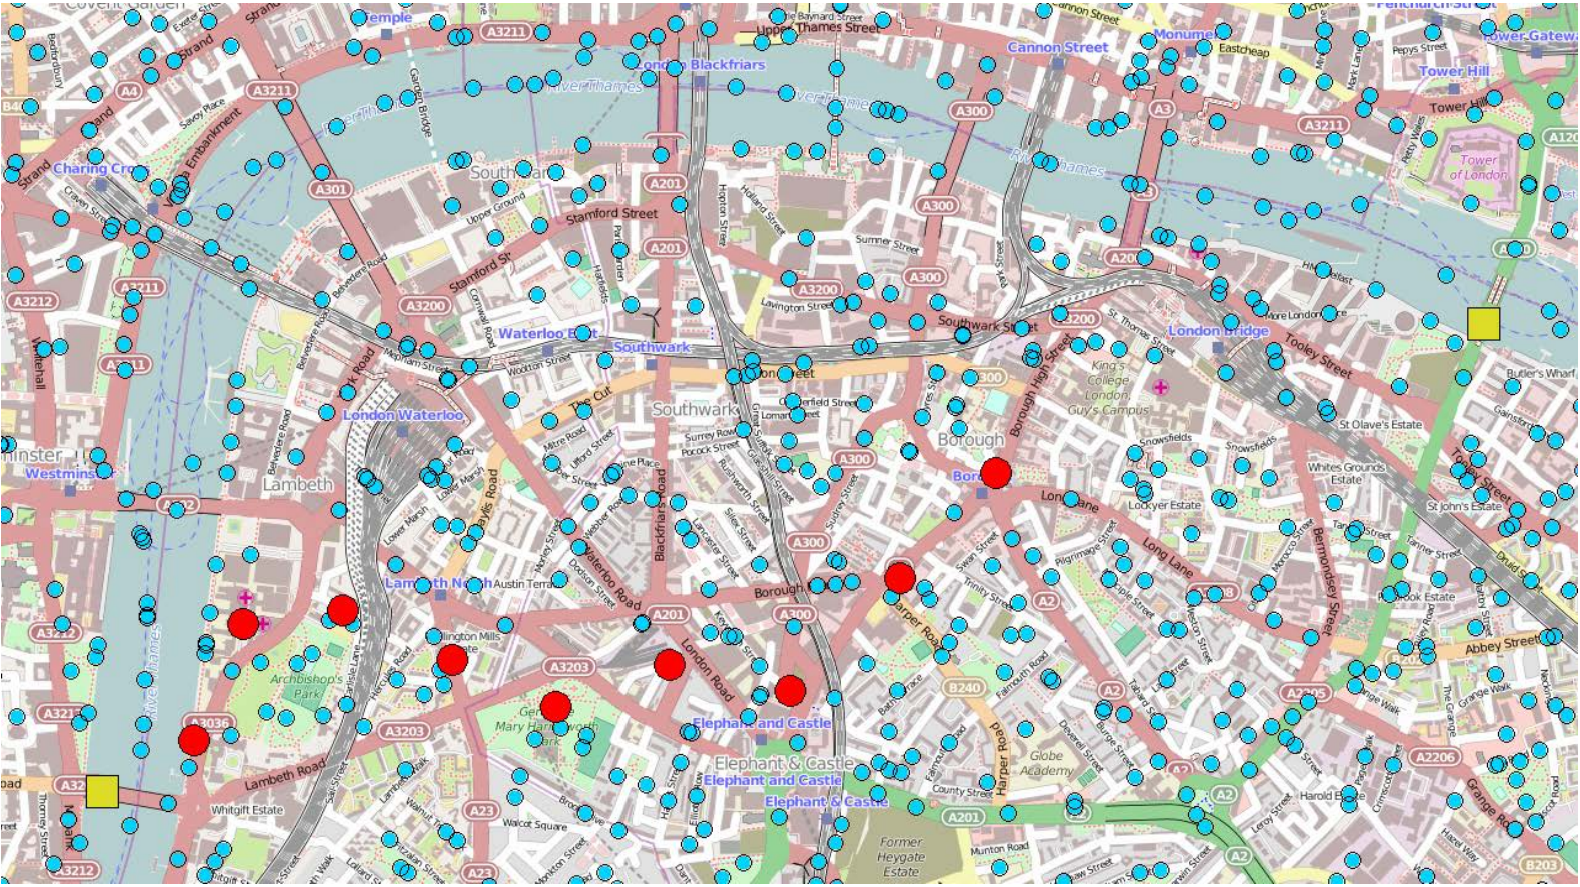
\includegraphics[width=\textwidth]{figures/protelis-example-c.png}
        \caption{Path continues to extend.}
        \label{fig:protelis-example-c}
    \end{subfigure}
    \hfill
    \begin{subfigure}[b]{.49\textwidth}
        \centering
        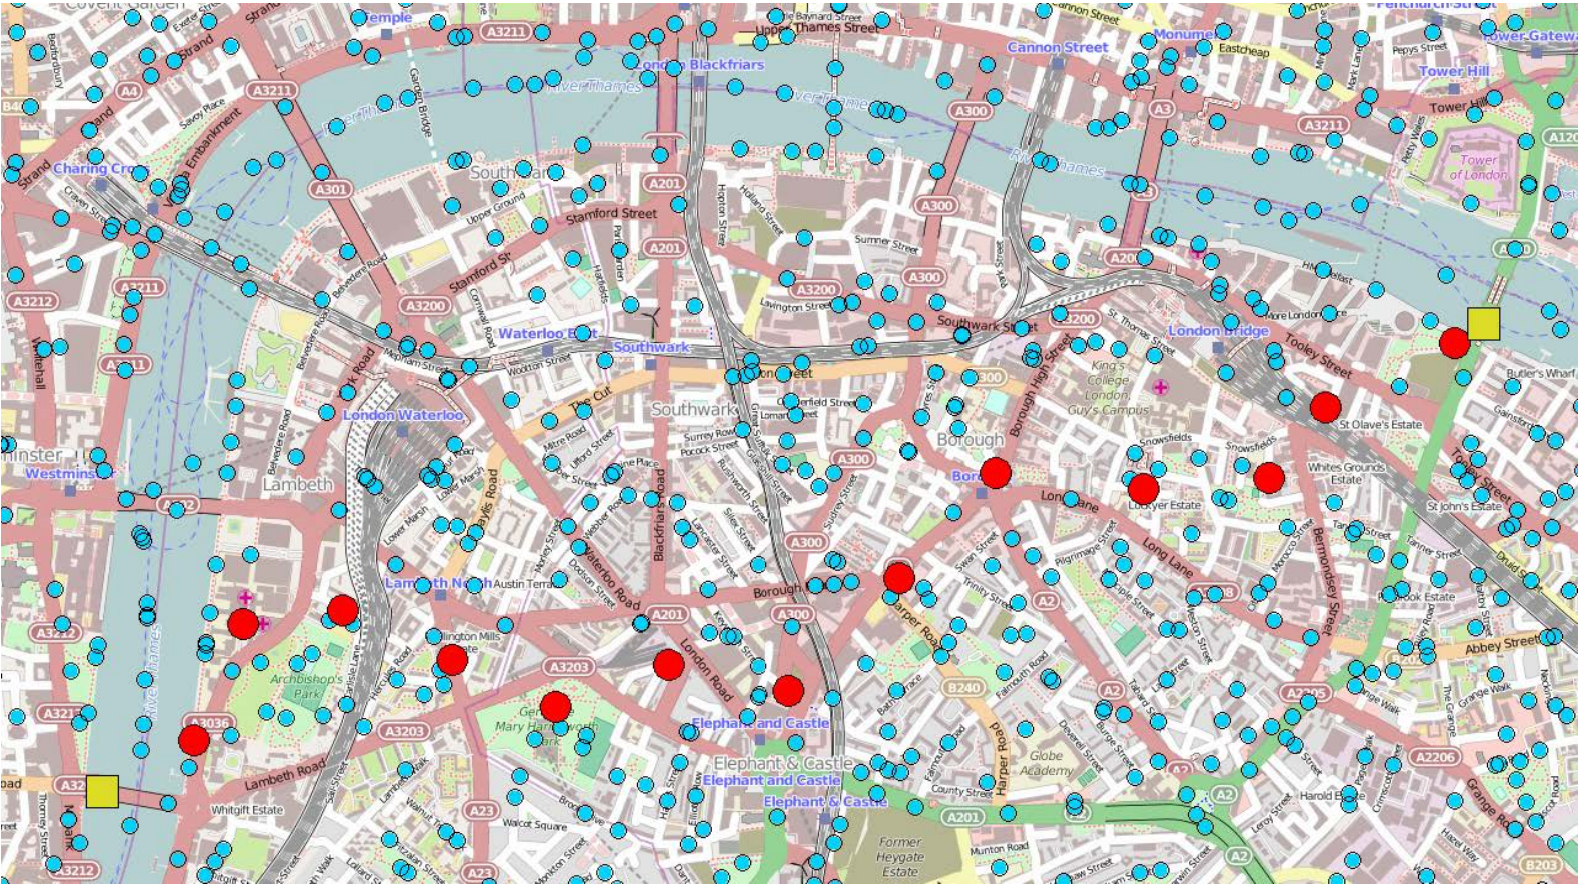
\includegraphics[width=\textwidth]{figures/protelis-example-d.png}
        \caption{Path computation complete.}
        \label{fig:protelis-example-d}
    \end{subfigure}
    \caption{Example of computing a rendezvous route for two people in a crowded urban environment.}
    \label{fig:protelis-example-map}
\end{figure}


\subsection{ScaFi}

ScaFi~\cite{Casadei2022} is a Scala-based library and framework designed for aggregate programming. It facilitates the development of distributed algorithms where computations are performed by individual devices in a network, and the results are aggregated across the network. The core concepts and constructs of ScaFi's API are outlined as follows:

\paragraph{Expression Evaluation}
An expression written using the ScaFi API is evaluated by each device once per computation round.

\paragraph{Fields}
Fields are represented as atomic values without any particular wrapper. They indicate the value of the field at the device performing the computation.

\paragraph{Neighboring Field}
The concept of ``neighboring field" from field calculus is not explicitly represented (not reified). Spatial computation (\texttt{nbr} and \texttt{nbrvar} constructs) is only available inside a special scope provided by the \texttt{foldhood} construct.

\paragraph{Export}
The export for each iteration is constructed by the ScaFi engine. It applies side effects to an internal data structure as the constructs are invoked, thereby constructing the evaluation tree.

\paragraph{Constructs}
The semantics of the constructs defined in ScaFi are described below:
\begin{itemize}
    \item \texttt{rep(init)(f)}: captures state evolution, starting from an \texttt{init} value that is updated each round through \texttt{f};
    \item \texttt{nbr(e)} captures communication, of the value computed from its \texttt{e} expression, with neighbors; it is used only inside the argument \texttt{expr} of \texttt{foldhood(init)(acc)(expr)}, which supports neighborhood data aggregation, through a standard “fold” of functional programming with initial value \texttt{init}, accumulator function \texttt{acc}, and the set of values to fold over obtained by evaluating expr against all neighbors;
    \item \texttt{branch(cond)(th)(el)} captures domain partitioning (space-time branching): essentially, the devices for which \texttt{cond} evaluates to \texttt{true} will run sub-computation \texttt{th}, while the others will run \texttt{el};
    \item \texttt{mid} is a built-in sensor providing the identifier of devices;
    \item \texttt{sense(sensorName)} abstracts access to local sensors;
    \item \texttt{nbrvar(sensorName)} abstracts access to “neighboring sensors” that behave similarly to \texttt{nbr} but are provided by the platform: i.e., such sensors provide a value for each neighbor.
\end{itemize}

\subsubsection{Gradient Implementation in ScaFi}

A \textit{(self-healing) gradient} is a distributed behavior that self-stabilizes, in each device of the distributed system, to a value denoting its minimum distance from the closest source node (for instance, computed by summing the neighbor-to-neighbor distances along the shortest path to the source), adapting to changes in the source set and distances. By following the neighbors of maximum decrease (resp. increase) of the gradient value, i.e., by descending (resp. ascending) the gradient, it is possible to implement efficient hop-by-hop information flows, that can be useful for data propagation and collection.

The implementation of a gradient using ScaFi is presented in \Cref{lst:scafi-gradient}. The following is a brief description of the program:
The gradient value at each node is dynamically evolved using \texttt{rep}. This is necessary to allow a node to share its previous gradient value with neighbors. The default value is \texttt{Double.PositiveInfinity} since by default a node is at an infinite distance from a source (since it may not be reachable in general). The \texttt{mux(c)(th)(el)} evaluates its expression \texttt{th} and \texttt{el} and then uses the Boolean condition \texttt{c} to select either the former (when \texttt{c} is true) or the latter (when \texttt{c} is false).
If a node is a source (i.e., if sensing the Boolean sensor \texttt{source} returns \texttt{true}), then its gradient value is \texttt{0} (by definition).
If a node is not a source, then will take as its gradient value the output of the expression \texttt{minHoodPlus(nbr\{distance\} + nbrRange)}.
\texttt{minHoodPlus(e)} is a variant of \texttt{foldhood} which does not consider the device itself when folding over the neighborhood. Namely, it selects the minimum value among those obtained by evaluating \texttt{e} against the neighbors. The argument of \texttt{minHoodPlus} is \texttt{nbr\{distance\} + nbrRange()}, which amounts to calculating, for each neighbor, the sum of the neighbor's most recent gradient value and the corresponding distance to that neighbor (obtained by neighboring sensor \texttt{nbrRange}, which is \texttt{nbrvar[Double]("nbrRange")}).

\lstinputlisting[float,label={lst:scafi-gradient},language=scala,caption=Implementation of gradient in ScaFi]{listings/scafi-gradient.scala}

\begin{figure}
    \centering
    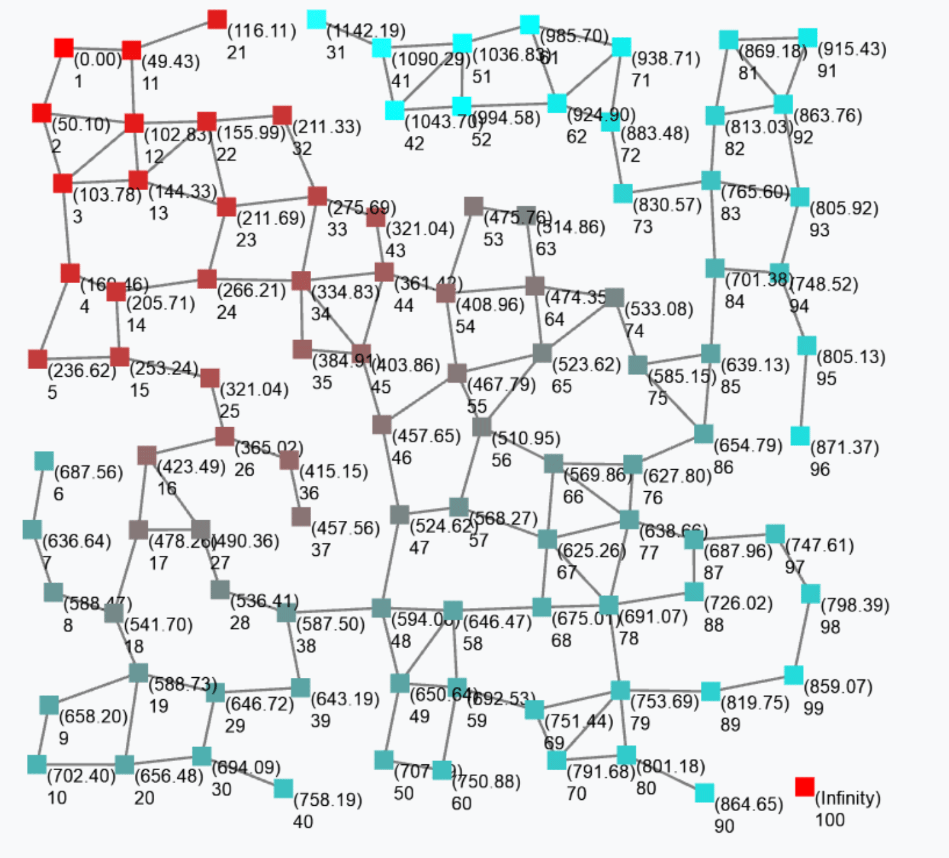
\includegraphics[width=\linewidth]{figures/scafi-gradient.png}
    \caption{A graphical representation of the gradient implementation in ScaFi after stabilization. Each device of the network is labeled with its distance from the source (in parenthesis) and its ID. The source device is the one with ID 1. Note that devices that are not connected to the source are considered to be at an infinite distance from it.}
    \label{fig:scafi-gradient}
\end{figure}

\subsection{FCPP}

FCPP~\cite{Audrito2020} is a C++14 library implementing Field Calculus and providing tools for distributed system simulation.

Its extensible component-based architecture allows customization for diverse application scenarios, such as Internet-of-Things (IoT) deployments, simulations, and self-organizing cloud applications. Users can add components tailored to specific functionalities, enhancing flexibility and applicability. The library incorporates compile-time optimizations and supports parallel execution, enabling efficient simulation of both systems and self-organizing cloud applications. Currently, FCPP focuses on distributed system simulations but already significantly reduces simulation costs, accelerating the development of new distributed algorithms. These features offer a path for a convenient extension to address previously ineffective scenarios:

Existing implementations often have high-performance requirements, unsuitable for resource-constrained microcontrollers. FCPP's lightweight nature makes it well-suited for these systems.

Self-organizing cloud applications necessitate fine-grained parallelism for scalability, and performance improvements directly translate to cost reduction. FCPP's support for parallelism caters to this need.

\subsubsection{Aggregate Program Example with FCPP}

The example function provided in \Cref{lst:fcpp-example} utilizes the Adaptive Bellman-Ford algorithm to estimate distances from devices where the \texttt{source} parameter is \texttt{true}. This function explicitly takes a \texttt{node} object as input, enabling access to its functionalities, including the \texttt{nbr\_dist()} method. This method returns a \texttt{field<double>} representing the estimated distances to neighboring nodes.

The \texttt{call\_point} parameter serves two purposes:

\begin{itemize}
    \item Updating the \texttt{node.stack\_trace} (shared functionality across all aggregate functions, as noted in the first line).
    \item Facilitating the aggregation of function calls (e.g., \texttt{nbr} and \texttt{min\_hood}) by providing an incrementing index.
\end{itemize}

\lstinputlisting[float,label={lst:fcpp-example},language=C++,caption=Implementation Adaptive Bellman Ford algorithm in FCPP]{listings/fcpp-example.cpp}

\subsection{Collektive}

Collektive\footnote{\url{https://github.com/Collektive/collektive}} provides the user with a DSL, implemented in Kotlin, that allows to create aggregate programs transparently. It was designed with the following principles in mind: transparency, minimality and portability.

Transparency refers to the clear and concise information it provides about how the underlying system behaves, such as data processing, storage, and communication between nodes. Transparency helps to reduce complexity, making it easier to understand and maintain large and complex systems.

Collektive is designed with the fewest possible constructs and abstractions while still offering the required functionalities. This reduces the complexity of the system, making it easier to maintain and debug, and lowers the overhead associated with using the DSL, which is particularly important for systems that require high performance and scalability.

Portability refers to its ability to run on various platforms and environments, including different operating systems, cloud platforms, and hardware architectures. This enables systems built with the DSL to be easily deployed and run in different environments, which is crucial for systems requiring deployment in multiple locations or scalability to meet changing demands.

Constructs implemented in Collektive are defined in \Cref{lst:collektive-constructs}, while the semantics are described below:

\begin{itemize}
    \item \texttt{exchange}~\cite{https://doi.org/10.4230/lipics.ecoop.2022.20}: manages the computation of values between neighbors in a specific context. It computes a \texttt{body} function starting from the \texttt{initial} value and the messages received from other neighbors, then sends the results from the evaluation to specific neighbors or everyone, it is contingent upon the origin of the calculated value, whether it was received from a neighbor or if it constituted the initial value. The result of this function is a field with as messages a map with as key the ID of the devices across the network and the result of the computation passed as relative local values.
    \item \texttt{exchanging}: Same behavior of \texttt{exchange} but this function can yield a \texttt{Field} of \texttt{Return} value.
    \item \texttt{repeat}: Iteratively updates the value computing the \texttt{transform} expression at each device using the last computed value or the \texttt{initial}.
    \item \texttt{repeating}: Iteratively updates the value computing the \texttt{transform} expression from a \texttt{YieldingContext} at each device using the last computed value or the \texttt{initial}.
\end{itemize}

\lstinputlisting[float,label={lst:collektive-constructs},language=kotlin,caption=Base constructs implemented in Collektive]{listings/collektive-constructs.kt}

\subsubsection{Example of Gradient in Collektive}

In the \Cref{lst:collektive-gradient}, the implementation of the gradient in Collektive is presented. In this case, it is used a construct that is not strictly part of the field calculus but extends it; it is the \texttt{share} construct~\cite{https://doi.org/10.48550/arxiv.1910.02874}. \texttt{share} captures the space-time nature of field computation through observation of neighbors' values, starting from an \texttt{initial} value, it reduces to a single local value given a \texttt{transform} function and updating and sharing to neighbors of a local variable.

\lstinputlisting[float,label={lst:collektive-gradient},language=kotlin,caption=Gradient implementation in Collektive]{listings/collektive-gradient.kt}

\subsection{FRASP}

As said in \Cref{subsection:reactive-and-proactive-models}, aggregate computing makes use of a round-based execution model, that can be defined as proactive. This approach is simple to reason about but limited in terms of flexibility in scheduling and management of sub-activities (and response to contextual changes). In~\cite{Casadei2023} is proposed a reactive self-organization programming approach, called FRASP, that enables the decoupling of the program logic from the scheduling of its sub-activities. This model maintains the same expressiveness and benefits of aggregate programming while enabling significant improvements in terms of scheduling controllability, flexibility in the sensing/actuation model, and execution efficiency.

\subsubsection{Reactive Model}
FRASP is based on the functional reactive programming (FRP) paradigm and considers \textit{continuous time}, $Time$ = $\{ t \in \mathbb{R} \, | \, t \geq 0 \}$. Time-varying values are called \textit{cells} and may be conceptually modeled by generic functions of type $Cell$ $a$: $Time \rightarrow a$. Then, \textit{streams} are discrete-time values and may be modeled by generic functions of type $Stream$ $a$: $[Time] \rightarrow [a]$, namely, mapping a sequence of (increasing) sample times to a sequence of corresponding values. While cells model state, streams model state changes.

\subsubsection{Abstractions and Primitives}

One of the main differences between the proactive and reactive models is that the latter allows the self-organizing collective computation to be expressed as a graph of reactive sub-computations. Each sub-computation is called \textit{flow} and represents it programmatically through type \texttt{Flow[T]}, where \texttt{T} is the type of the output of the wrapped computation. A \texttt{Flow} is essentially a function that takes a \texttt{Context} and returns a cell of \texttt{Export}s, possibly depending on the exports of other \texttt{Flow}s, recursively.

The details of the syntax and semantics of FRASP are discussed in detail in Section III of~\cite{Casadei2023} while in this section they are presented in a simplified manner:

\begin{itemize}
    \item \texttt{constant(e)} returns a constant flow that always evaluates to the argument that has been passed;
    \item \texttt{sensor(name)} returns the flow of values produced by the sensor with the given \texttt{name};
    \item \texttt{mid()} returns the constant flow of the device ID;
    \item \texttt{mux(c)\{t\}\{e\}} is an expression that returns a flow with the same output of flow \texttt{t} when the Boolean flow \texttt{c} is true and the output of flow \texttt{e} when \texttt{c} is false;
    \item \texttt{nbr(f)} handles communication with neighbors in both directions at once, it takes a flow \texttt{f} as a parameter;
    \item \texttt{branch(c)\{t\}\{e\}} evaluates and returns the value of expression \texttt{t} when \texttt{c} evaluates to true. This enables a form of distributed branching, where devices that happen to execute \texttt{t} will not interact with those that executed \texttt{e} (and vice versa);
    \item \texttt{loop(init,ft)} evolves a piece of state (initially, \texttt{init}) by applying function \texttt{ft} mapping the previous state's flow to the next state's flow.
\end{itemize}

\subsubsection{Gradient Implementation in FRASP}

\Cref{lst:frasp-gradient} provides a representation of a gradient in FRASP. The function takes the Boolean \texttt{src} flow as input, denoting whether the executing node is the source of the gradient or not. The external \texttt{loop} is used to progressively evolve the current gradient value \texttt{distance} starting from an infinite value (as, initially, devices do not know whether a source is reachable). Internally to the loop, \texttt{mux} is used to select one of two values: if the node is a source, then its gradient value is \texttt{0} (base case); otherwise, the gradient should be the minimum value among the neighbors' gradient values augmented by the distance (\texttt{nbrRange}) from that very neighbor. Construct \texttt{liftTwice} is used to combine (using the sum: \_+\_) the two flows \texttt{nbrRange} (distances to neighbors) and \texttt{nbr(distance)} (neighbors' gradient values).

\lstinputlisting[label={lst:frasp-gradient},language=scala,caption=Gradient implementation in FRASP]{listings/frasp-gradient.scala}

The reactive dataflow graph in \Cref{fig:gradient-dependencies} corresponds to \Cref{lst:frasp-gradient}. \Cref{fig:gradient-dependencies} provides the local view of the computation for a single node (where the layers denote different semantic kinds of dependencies), whereas \Cref{fig:gradient-dependencies-distributed} shows the distributed dependency graph. The arrows denote dependencies. The dashed arrows denote dependencies based on platform-level scheduling and node interaction; for instance, a red block depends on changes corresponding to neighbors' red blocks and is communicated via message passing.

\begin{figure}
    \centering
    \begin{subfigure}[b]{\textwidth}
        \centering
        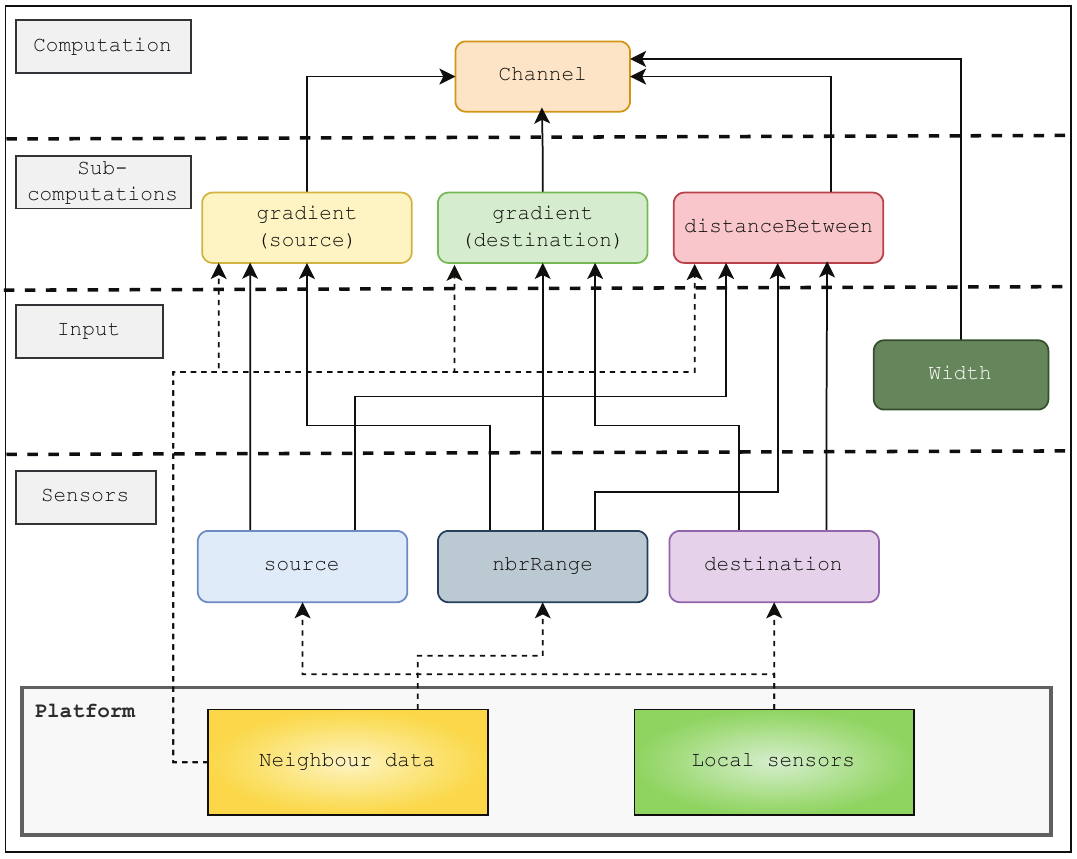
\includegraphics[width=\textwidth]{figures/gradient-dependencies.png}
        \caption{Node view.}
        \label{fig:gradient-dependencies}
    \end{subfigure}
    \hfill
    \begin{subfigure}[b]{\textwidth}
        \centering
        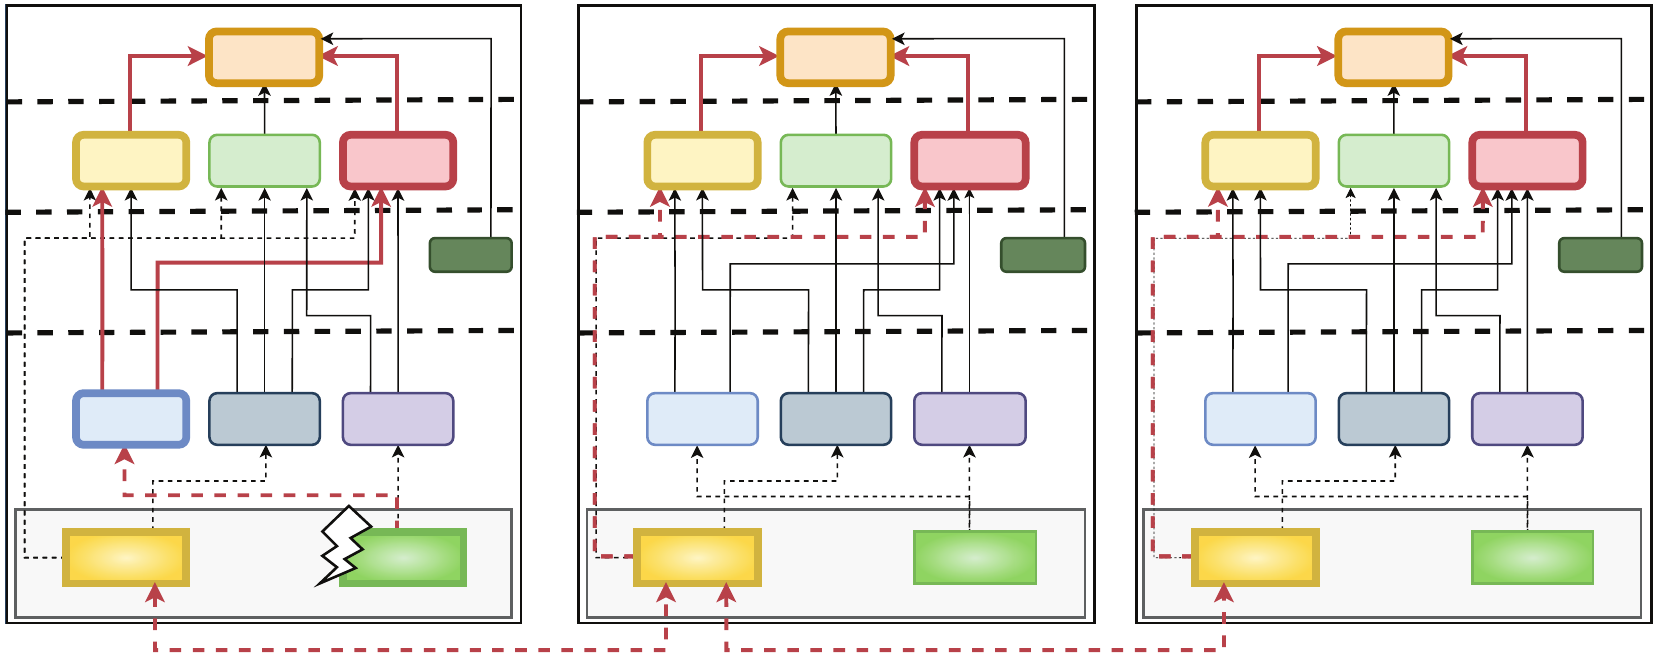
\includegraphics[width=\textwidth]{figures/gradient-dependencies-distributed.png}
        \caption{Distributed view (with neighbor dependencies).}
        \label{fig:gradient-dependencies-distributed}
    \end{subfigure}
    \caption{Dependencies between sub-computations in gradient program (\Cref{lst:frasp-gradient})}
\end{figure}

\section{Design of FRASP}

\subsection{Architecture}

\begin{figure}
    \centering
    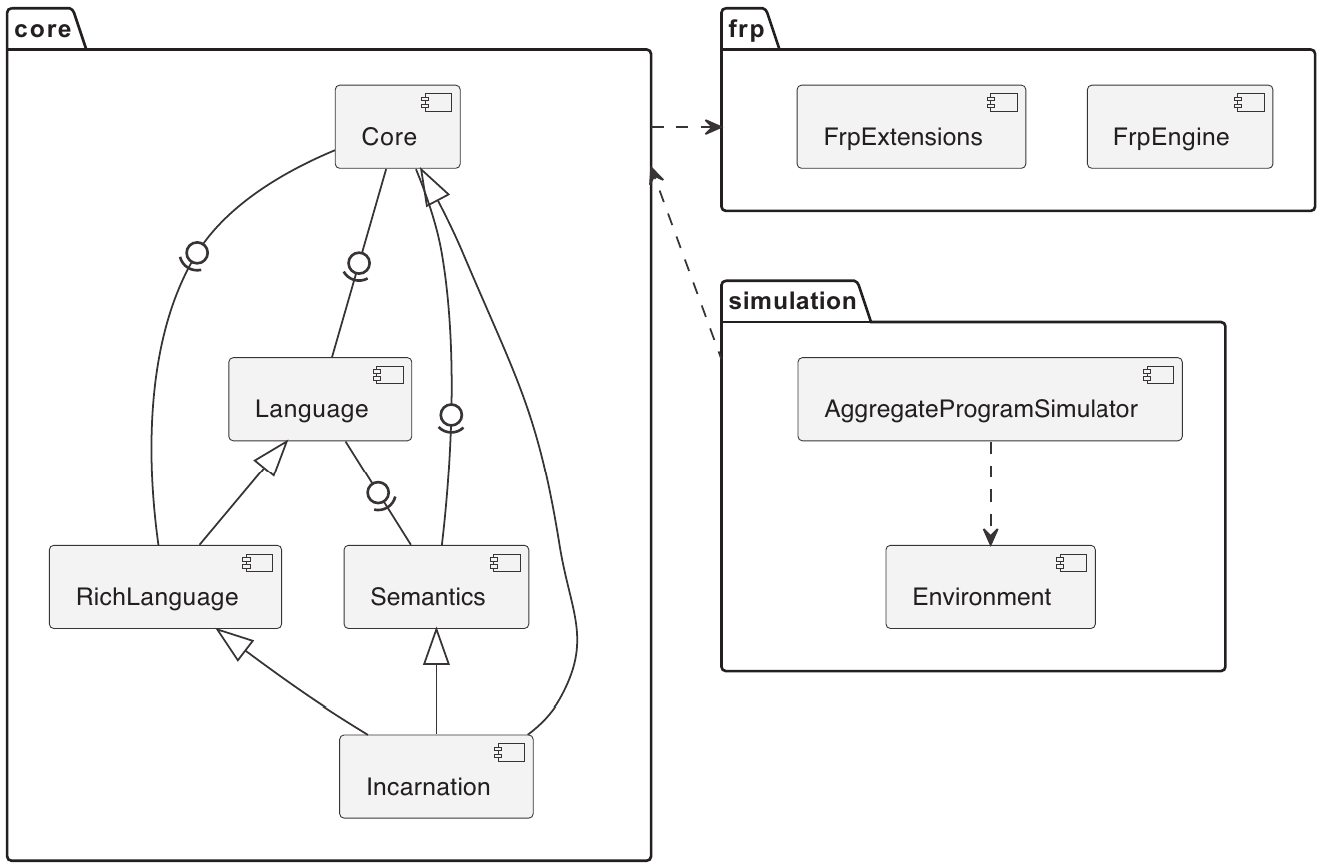
\includegraphics[width=\linewidth]{figures/FRASP-architecture.png}
    \caption{FRASP architecture.}
    \label{fig:frasp-architecture}
\end{figure}

\subsection{Detailed Design}

\begin{figure}
    \centering
    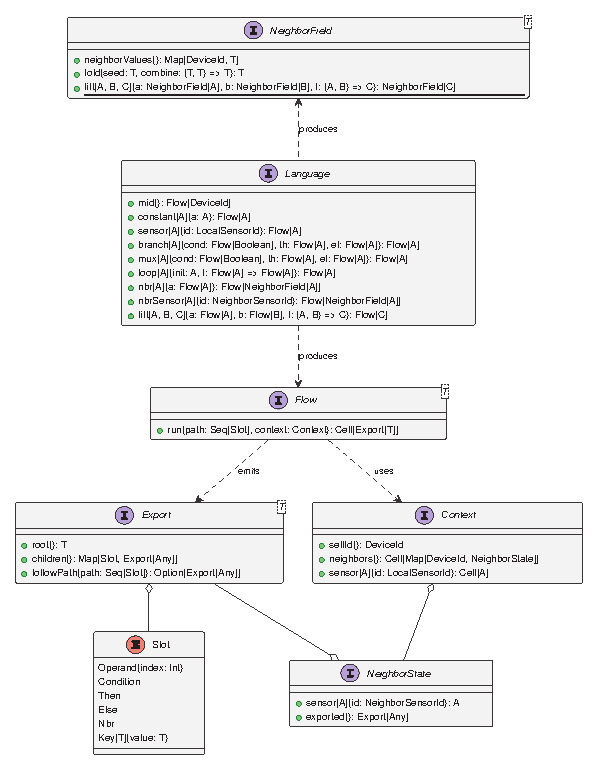
\includegraphics[width=\linewidth]{figures/FRASP-design.pdf}
    \caption{FRASP detailed design.}
    \label{fig:frasp-design}
\end{figure}

\section{Design of Collektive}

\subsection{Architecture}

\subsection{Detailed Design}

\section{Integration of FRASP in Collektive}